\subsection{Autocorrelation of the Idle periods - Results} \label{sec:autocorrelation_idle_results}
Here we performed different tests for the \acs{K-S} in order to study the independence of the samples. The \acs{K-S} uses the idle samples in order to perform a fitting test of the empirical distribution (generated by the simulation) and the estimated distribution (constructed from the parameters obtained in the estimation process). The \acs{K-S} requires that the samples used for the test need to be independent. Here we studied the independence of these samples.

We simulated 100 runs of one of the experiments (medium-load case) of Section \ref{sec:ks-results} and extracted the P-value failure rate and the sequence of idle samples. The experiment results gave us a $P(P-value<0.1)$ of 14\% (see Figure \ref{fig:autocorrelation_cdf_p_normal}) and we obtained and represented the autocorrelation function of the samples. As it can be observed in Figure \ref{fig:autocorrelation_idle_normal}, the correlation of the idle samples is low.

\begin{figure}[h!]
	\centering
	\subfloat[]{
		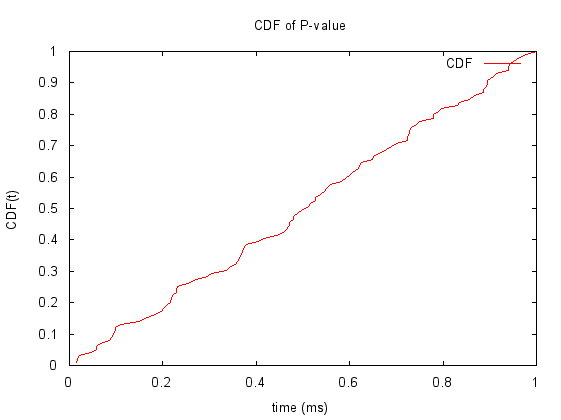
\includegraphics[width=0.45\textwidth, trim = 0mm 0mm 0mm 0mm, clip]{images/results/autocorrelation/ks_samples/cdf_p_normal}
		\label{fig:autocorrelation_cdf_p_normal}
	}
	\subfloat[]{
		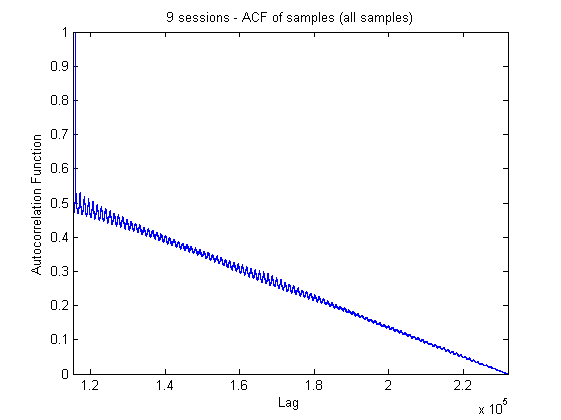
\includegraphics[width=0.45\textwidth, trim = 0mm 0mm 0mm 0mm, clip]{images/results/autocorrelation/ks_samples/normal}
		\label{fig:autocorrelation_samples_normal}
	}
	\caption{P-value failure rate and autocorrelation of the idle samples}
	\label{fig:autocorrelation_idle_normal}
\end{figure}

In order to try to have a better independence between samples, we decided to gather more separated samples for the \acs{K-S} and see if the independence is increased, and in extension, the p-value failure rate is improved. The results are represented in Figure \ref{fig:autocorrelation_idle_reduced13} and Figure \ref{fig:autocorrelation_idle_reduced15}.

\begin{figure}[h!]
	\centering
	\subfloat[]{
		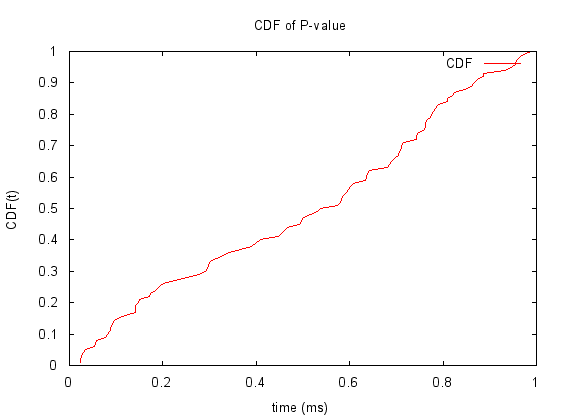
\includegraphics[width=0.45\textwidth, trim = 0mm 0mm 0mm 0mm, clip]{images/results/autocorrelation/ks_samples/cdf_p_reduced-1-3}
		\label{fig:autocorrelation_cdf_p_reduced13}
	}
	\subfloat[]{
		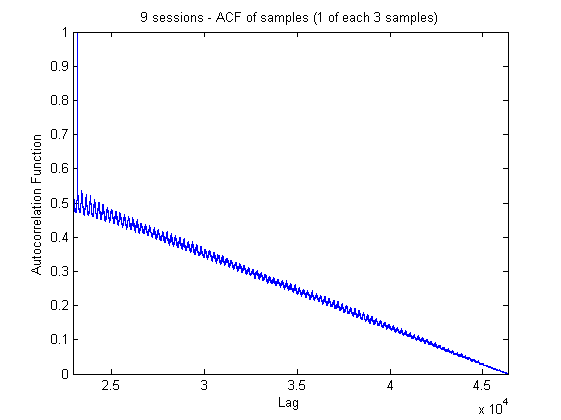
\includegraphics[width=0.45\textwidth, trim = 0mm 0mm 0mm 0mm, clip]{images/results/autocorrelation/ks_samples/reduced-1-3}
		\label{fig:autocorrelation_samples_reduced13}
	}
	\caption{P-value failure rate and autocorrelation of the idle samples using 1 every 3 samples}
	\label{fig:autocorrelation_idle_reduced13}
\end{figure}

\begin{figure}[h!]
	\centering
	\subfloat[]{
		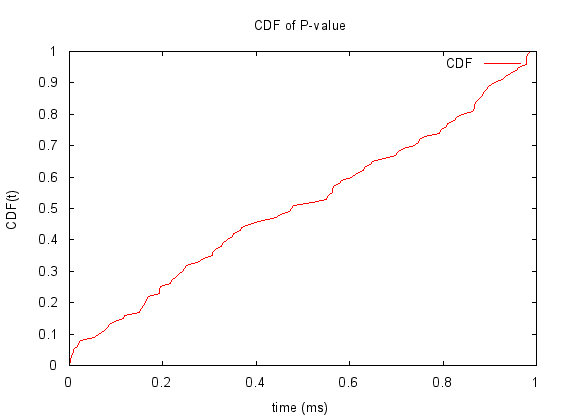
\includegraphics[width=0.45\textwidth, trim = 0mm 0mm 0mm 0mm, clip]{images/results/autocorrelation/ks_samples/cdf_p_reduced-1-5}
		\label{fig:autocorrelation_cdf_p_reduced15}
	}
	\subfloat[]{
		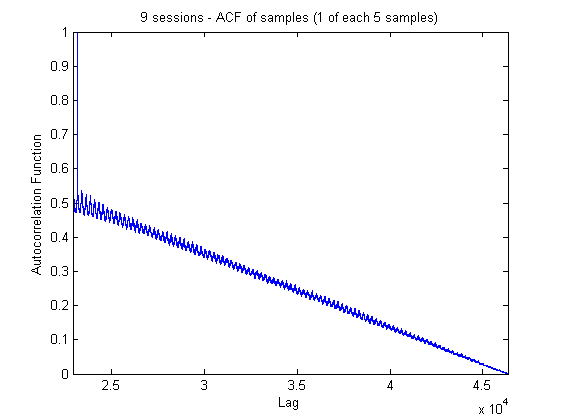
\includegraphics[width=0.45\textwidth, trim = 0mm 0mm 0mm 0mm, clip]{images/results/autocorrelation/ks_samples/reduced-1-5}
		\label{fig:autocorrelation_samples_reduced15}
	}
	\caption{P-value failure rate and autocorrelation of the idle samples using 1 every 5 samples}
	\label{fig:autocorrelation_idle_reduced15}
\end{figure}

We separated the number of samples using one every three or one every five idle samples for the \acs{K-S} test. As it can be observed from the autocorrelation function of the idle samples of each one of the cases (Figure \ref{fig:autocorrelation_samples_reduced13} and \ref{fig:autocorrelation_samples_reduced15}) the independence of the samples is still the same as the normal case (Figure \ref{fig:autocorrelation_samples_normal}), which means that using a set of more separated samples, it is not possible to improve the independence of the samples. In extension, there is no improvement of the p-value failure rate in the \acs{K-S} (Figures \ref{fig:autocorrelation_cdf_p_reduced13} and \ref{fig:autocorrelation_cdf_p_reduced15}), which give us similar results as the normal case in Figure \ref{fig:autocorrelation_cdf_p_normal} (around 12-14\%). Then, our validation test is already using a set of independent samples that cannot be improved by this method.

We can conclude then, that the independence of the idle samples used for the validation test cannot be improved more even using more separated samples. So we still are facing the same problem as in Section \ref{sec:ks-results} that made us reconsider if the \acs{K-S} as the proper validation test for our model.

%TODO:
%Gather more separated samples: separation of 10, 100 samples and add the results.
